\subsection{Authenticity}
We have found a way to encrypt messages, meaning no one can see our messages from outside, but in the first place we have to make sure that our messages go to the right persons and vis versa, we need to be able to be sure that the message we have received is from the right person. Do to do, one need to define \important{authenticity}. 
\begin{definition}{(Authentication)}
	The process of verifying a claimed identity.
\end{definition}
\begin{parag}{Ways to prove who you are}
    Traditionally, we have a lot of methods in order to authenticate ourself :
	\begin{itemize}
	    \item \textbf{What you know}: password, secret key
	    \item \textbf{What you are}: biometrics
	    \item \textbf{What you have}: smart card, secure token
	\end{itemize}
	However now what can use many other ways to prove :
	\begin{itemize}
	    \item \textbf{Where you are}: location, IP address
	    \item \textbf{How you act} behavioural authentication
	    \item \textbf{Who you know}: social ties
	    \item $\vdots$
	\end{itemize}
	
	
\end{parag}

\begin{parag}{Public key cryptography}
    To go back on public key cryptography, the way it worked was that we needed a public key infrastructure which allowed us to expose our public keys to the world in order to communicate. To do so we need \important{digital signature}, \important{signing} and \important{verification}. The public key infrastructure needs to ensure authenticity. \\
	$ $\\
	Imagine now that Bob (secret key $SK$, public key $PK$) and Bob wants to communicate, he will send a message $M$ and also a \important{signing} defined as
	\begin{align*} 
		\text{Sign}_{SK}\left(M\right) = S 
	\end{align*}
	and send this back to Alice which she can verify using here own function $V_{PK}$
	\begin{align*} 
		V_{PK}\left(M, S\right) =  \checkmark
	\end{align*}
	\begin{center}
	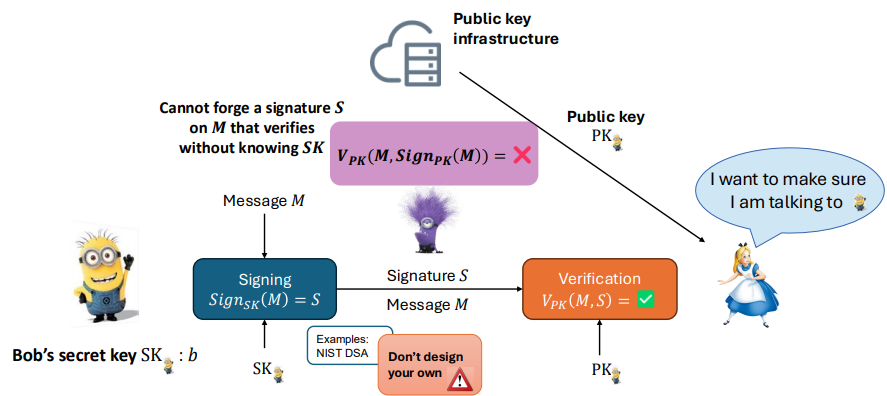
\includegraphics[scale=0.4]{screenshots/2026-10-15.png}
	\end{center}
\end{parag}
So how it works is the following 
\begin{itemize}
    \item Bob has a secret key. Using this key Bob performs a \important{digital signature} on the message.
    \item To verify a signature, Alice get Bob's public key from the repository and performs a verification function using the message, the signature, and Bob's public key. This function returns yes if the signature is valid, and no otherwise.
\end{itemize}
    To be secure, and provide integrity, Digital Signature algorithms need to be such that it is not possible to create a Signature for a message that will verify under a given public key, unless you have the corresponding secret key. Under these properties, a digital signature enable Alice to know that she is talking to Bob: only Bob, that knows the secret key, could have created the signature.

\begin{parag}{Digital signatures}
    Digital signatures are computationally costly compared with most symmetric key algorithms of equivalent security, what this means concretely is that signing and encrypting is \important{slow} (not having to pre-share a key comes at a cost).\\
	$ $\\
	Naively, this gives us a big issue, having long message implies that the signing and verification will take a very long time and will be not practical, if you remember CS-200, you may remember the way to solve that issue :
\end{parag}
\subsection{Hash Functions}
\label{par:Hash functions}
Hence, let us define three security properties that a hash function require
\begin{itemize}
    \item \textbf{Pre-image resistance}: Given $H =  h\left(M\right)$, it should be difficult to find $M$
    \item \textbf{Second Pre-image resistance}: Given $M$, difficult to find $M' \neq M$ such that $h\left(M'\right) = h\left(M\right)$
    \item \textbf{Collision Resistance}: difficult to find any $M, M'$ such that $h\left(M\right) =  h\left(M'\right)$
    \item \textbf{Deterministic}: Given $M$ a hash function $H$ will always output the same string $h =  H\left(M\right)$
\end{itemize}
Cryptographic hash functions are designed to be fast and efficient to compute, and they have several important properties that make them valuable in various applications.

\begin{figure}[h!]
\centering
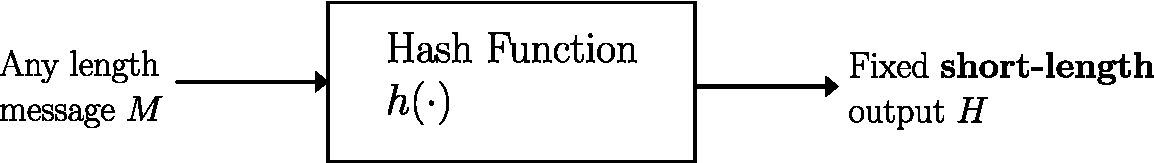
\includegraphics[width=0.8\textwidth]{figure/2026-10-15.pdf}
\caption{A beautiful diagram of a hash function (right?)}
\end{figure}

As always, one should never design those themselves and should use already existing hash functions 
\begin{itemize}
    \item MD5 (1991): 128 bits hash --- insecure
    \item SHA0, SHA1: 160 bits --- insecure
    \item SHA-2 (224/256 /384/512) --- Ok but slow
    \item SHA-3 (224/256 /384/512)
\end{itemize}
The use cases of hash function are vast, in order to support digital signatures, build HMAC, password storage, file integrety, secure commitments, secure logging, blockchains, ...


\begin{parag}{Digital signatures on hash functions}
	So now instead of having a digital signature on the whole message (which can be enormous), one can sign using the \important{hash} of the message. Meaning that instead of having $\text{Sign}_{SK}\left(M\right) =  S$, we will replace $M$ by $H = h\left(M\right)$. Alice on the other side will receive both the signature and the message and also need to compute the hash of the message on her side in order to apply the verification.\\
	$ $\\
    So how it works is the following: only Bob has his secret key $SK$, so only Bob can produce a signature $S$ that verifies under his public key $PK$. When Alice checks $V_{PJ}\left(h\left(M\right), S\right) = \checkmark$, she learns two things:
	\begin{itemize}
	    \item \important{origin}: the signature was made by whoever holds Bob's $SK$, which should be Bob
	    \item \important{Integrity}: $M$ wasn't modified. Changing $M$ changes $h\left(M\right)$, so the old signature no longer verified it.
	\end{itemize}
\end{parag}
\begin{framedremark}
Note that Preimage resistance is not needed here, as the message $m$ is already sent in public.
\end{framedremark}

\begin{parag}{All together}
    Now let us have both the encryption of the message and the signature so that we ensure, privacy and authentication. This implies that each users have \important{two pairs} of keys (2 $\times$ secret key, 2 $\times$ public key). In that case \important{confidentiality} is ensured as before with the ciphertext
	\begin{align*} 
		C = E_{PK}\left(M\right)
	\end{align*}
	and the decryption computed as 
	\begin{align*} 
	 	D_{SK}\left(c\right)
	\end{align*}
	$ $\\
	The authentication on the other hand is using the other pair of keys with
	\begin{align*} 
		 V_{PK}\left(M, S\right) = \checkmark \text{ with } S = \text{Sign}_{SK}\left(M\right)
	\end{align*}
	\begin{center}
	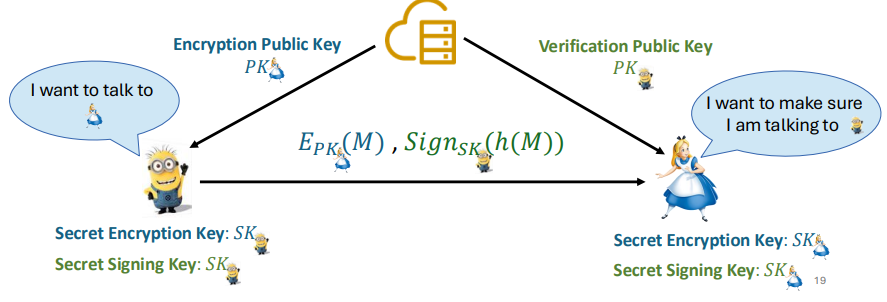
\includegraphics[scale=0.4]{screenshots/2026-10-15_1.png}
	\end{center}
\end{parag}


\subsection{Integrity}

Now we have again another problem \important{Integrity} 
\begin{definition}{(Integrity)}
information cannot be \important{modified} by unauthorized parties
\end{definition}

What this means is that if Bob sends '\textit{Banana}' he can be sure that Alice will receive '\textit{Banana}'.
\begin{parag}{Message integrity through digital signatures}
    As seen before in asymmetric cryptography, we have already seen a way to solve the integrity problem: digital signatures. Those provide 
	\begin{itemize}
	    \item Sender authenticity: since no party than the sender can create a valid signature for a message, the server can verify that the identity of the sender. No adversary can produce a valid signaature to the public key of the sender and therefore cannot impersonate the sender
	    \item Integrity of the message: Since no party than the sender can create a valid signature for a message, no adversary can modify the message without being detected (if they modify the message, the signature would not be valid)
	    \item Non-repudiation: Since no party than the sender can create a valid signature for a message, if a message has a valid signature, the sender cannot claim they did not sign it (no-one else can produce such signature).
	\end{itemize}
	However what this gives is that the signature $S$ only verified if message $M$ has not been modified
\end{parag}

\subsubsection{Integrity for Symmetric Cryptography}
    As in the asymmetric cryptography schemes, symmetric ones should also not have to suffer through integrity! Let us take the example of Block cipher,  meaning the message is sent by block of fixed size, typically 128/256 bits. What this implies is that in order to send a message of size greater than a block, we require iteration, which implies that we need to create some sort of mode operation:

\begin{parag}{Mode 1: Electronic Code Book (ECB)}
	Straightforward scheme: encrypt and decrypt single blocks. So we work as a '\textit{stream}' with each $M_i$ being encrypted with $E_K\left(\cdot \right) \to C_i$. For which we can then reconstruct the message as 
	\begin{align*} 
		M = M_1M_2M_3M_4\cdots 
	\end{align*}
	Which each block with the same size as the key. However we have a big issue here imagine that $M_i =  M_j$, what this gives is 
	\begin{align*} 
		M_i \to E_K\left(\cdot \right) \to C_i \\
		\underbrace{M_j}_{= M_i} \to E_K\left(\cdot \right) \to C_i
	\end{align*}
	\begin{center}
	    if $M_i = M_j$ then $C_i =  C_j$
	\end{center}
	which implies that the attacker learns something about the plaintext without breaking the cipher. Confidentiality means the ciphertext should reveal nothing about the message except its length. With ECB, it reveals which blocks are equal and that alone is often enough to learn a lot.
	
\end{parag}
\begin{parag}{Mode 2: Cipher Block Chaining (CBC)}
    The idea in this technique is to add some "\textit{noise}" in the encryption by block in order to '\textit{hide}' the equals blocks. We create an Initialization Vector (IV) which is a random block and the encrypt using the following rule 
	\begin{align*} 
		C_0 &=  IV\\
		C &= E_K\left(M_i \oplus C_{i-1}\right)
	\end{align*}
	\begin{center}
	\includesvg[scale=0.7]{figures/CBC_encryption.svg}
	\end{center}
	Where each block cipher encryption is $E_K\left(\cdot \right)$.
	\begin{subparag}{Remark}
	    Note that every time a block is encrypted, by the properties of the block cipher, the ciphertext is random. Because the IV and/or the plaintext changes every time, this random value is different every time. Thus, when XORed with the next plaintext it creates a random string. If the IV changes, this is similar to a one-block one-time pad, but if one reuses the IV for the same plaintext and key, this value will be repeated.
	\end{subparag}
\end{parag}
\begin{parag}{Decryption of CBC}
    In order to decrypt messages all we need to do is work the other way around. Recall that $C_0 =  IV$ and that $C_1 = E_K\left(M_1 \oplus IV\right)$. Decrypting it gives $D_K\left(C_1\right) = M_1 \oplus IV$ which means that we can recover $M_1$ as $M_1 =  M_1 \oplus IV \oplus IV$. Hence, given $C_i =  E_K\left(M_i \oplus C_{i-1}\right)$, Alice can decrypt it as $D_K\left(C_i\right) = M_i \oplus C_{i-1}$, by applying $\oplus C_{i-1}$ to it.
	\begin{align*} 
		M_i &= D_K\left(C_i\right) \oplus C_{i-1} \\
		&= M_i \oplus C_{i-1} \oplus C_{i-1}\\
		&= M_i
	\end{align*}
	However this raises some questions: what if $IV$ is incorrect? Is the full decryption wrong? Can you decrypt a block alone? What do you need?\\
	$ $\\
	If the IV is incorrect, only the first block is corrupted, Recall that the rest only depend on the ciphertext. Note also that blocks cannot be decrypted without having the previous ciphertext!
\end{parag}


\begin{parag}{Mode 3: Counter Mode (CTR)}
    The idea here it to use increasing nonce to add randomness without dependencies between block. What this means is that the CTR encryption is defined as 
	\begin{align*} 
		C_i =  E_K\left(\text{Nonce} + i\right) \oplus M_i 
	\end{align*}
	\begin{center}
	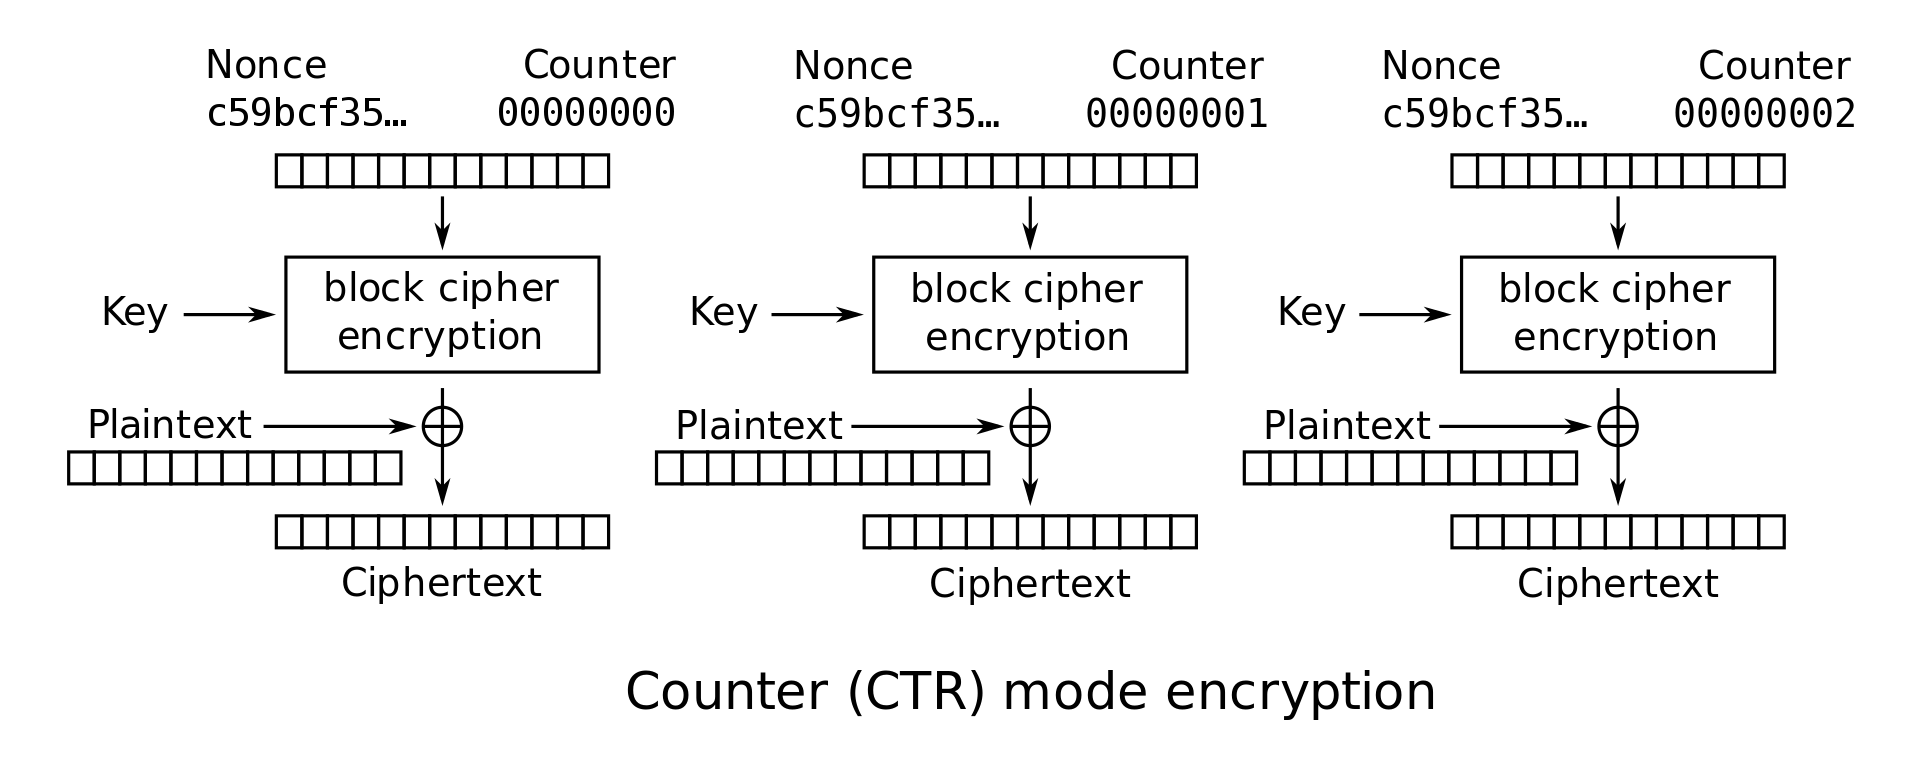
\includegraphics[scale=0.17]{screenshots/CTR_encryption.png}
	\end{center}
	Now the question is how do we decrypt this cipher? Well if you think about it:
	\begin{align*} 
		M_i = E_K\left(\text{Nonce} + i\right) \oplus C_i 
	\end{align*}
	right? Let us see if this is true 
	\begin{align*} 
		E_K\left(\text{Nonce} + i\right) \oplus C_i &= E_K\left(\text{Nonce} + i\right) \oplus E_K\left(\text{Nonce} + i\right) \oplus M_i\\
													&= M_i
	\end{align*}
\end{parag}
\begin{parag}{Block Ciphers}
    \begin{subparag}{Strengths}
        \begin{itemize}
            \item \textbf{High diffusion}: information from one plaintext symbol is diffused into several ciphertext symbols
            \item \textbf{Immunity to tampering}: difficult to insert symbols without detection
        \end{itemize}
    \end{subparag}
	\begin{subparag}{Weaknesses}
	    \begin{itemize}
	        \item \textbf{Slow}: an entire block must be accumulated before encryption/ decryption can begin
	        \item \textbf{Error propagation}: in some modes of operation errors affect several bits/blocks
	    \end{itemize}
	    
	\end{subparag}
\end{parag}

\paragraph{Summary}%
\label{par:Summary}

\begin{itemize}
    \item \textbf{Electronic Code Book (ECB)}: Directly encrypt and decrypt single blocks. Large information leakage due to lack of randomness across block's encryption
    \item \textbf{Cipher Block Chaining (CBC)}: Avoids ECB problems by using previous blocks to add randomness to every encryption. Propagates errors and prevents single-block decryption
    \item \textbf{Counter mode (CTR)}: Uses an increasing '\textit{nonce}' to introduce randomness across block's encryptions. Enable parallel encryption and decryption.
\end{itemize}

\paragraph{What about integrity?}%
\label{par:What about integrity?}
As in the asymmetric case, let us see how to ensure integrity for symmetric encryption. To do so we'll use \important{message authentication code} (\important{MAC}).
\begin{center}
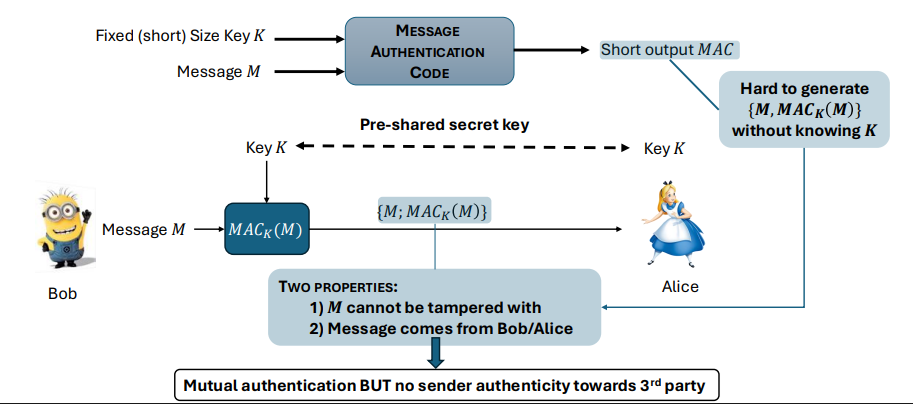
\includegraphics[scale=0.4]{screenshots/2026-10-15_2.png}
\end{center}
A MAC is like a hash function with a \important{key}. It takes a shared secret $K$ and a message $M$ and outputs a short tag $MAC_K\left(M\right)$. Alice computes $T =  MAC_K\left(M\right)$ and sends $\left\{M, T\right\}$. \\
$ $\\
Bob then receives $\left\{M, T\right\}$ and recomputes $MAC_K\left(M\right)$ himself using $K$, and checks whether it equals $T$.\\
$ $\\
But first let us be a bit more '\textit{formal}' about the defintion of our MAC. A message authentication code receives two inputs:
\begin{itemize}
    \item A small key that must be kept secret
    \item The message who integrity needs to be secured
\end{itemize}
The MAC algorithm outputs a short string that helps Alice to verify the integrity of the message sent by Bob.\\
$ $\\
The key property of the MAC is that it is very difficult to produce a pair [message; $MAC\left(k, \text{message}\right)$] without knowing the key.\\
$ $\\

This is the symmetric counterpart of a signature check. The difference is that Bob can't merely verify: he recomputes the exact same value, because he hols the same key. The integrity here comes from the fact that if Eve changes $M$, the tag no longer matches and she can't compute a new one without $K$. The authenticity on the other hand comes from that only someone who knows $K$ could have made the tag, so it came from Alice or Bob.
\begin{parag}{Repudiation}
    Now imagine an exchange between Alice and Bob with Charlie being a third party observes. Even though Alice and Bob know they are talking to each other (only any party with knowledge of $K$ could have produce a valid MAC, message pair, they both could have produced the message.)\\
	So the message can be repudiated which means both A and B can claim it was the other who wrote the message.
\end{parag}

\begin{parag}{Example MAC: CBC-MAC}
    Let us see how to turn a block cipher into a mac. To do so CBC MAC defines the following encryption methods 
	\begin{align*} 
		C_0 &= 0 [\text{ any fixed }IV] \\
		C_i &= E_K\left(M_i \oplus C_{i-1}\right)\\
		MAC_K\left(M_1 \ldots M_x\right) &=  C_n
	\end{align*}
	The difference here with CBC encryption is that CBC-MAC is deterministic, also only the output of CBC-MAC is the last block.
	\begin{subparag}{Remark}
	    Remark that CBC can be turned into a MAC by:\\
		$ $\\
		Fix $IV$ (e.g. 0) and then do CBC. The MAC is the output of the last encryption block: one could have only gotten there for one message and one key. Note that the last block cannot be used to recover anything about the message: it looks random (as it is the output of a block cipher)
	\end{subparag}
	\begin{subparag}{Limitation}
		The encryption scheme is only secure if the length of the message $M$ is known.
	\end{subparag}
	\begin{center}
	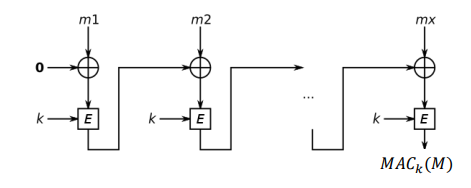
\includegraphics[scale=0.5]{screenshots/2026-10-15_3.png}
	\end{center}
\end{parag}

\paragraph{And all together now ...}%
\label{par:And all together now ...}

    \begin{parag}{Encrypt and MAC}
        \begin{itemize}
			\item $\times$ No integrity on the ciphertext $\to$ Cipher can be attacked which therefore mean that we need to decrypt to know if the ciphertext is valid
			\item \checkmark integrity of the plaintext can be verified
			\item $\times$ May reveal information about the plaintext $\to$ repeated messages, recall the $IV$ of the MAX is fixed (can be solved with a counter)
        \end{itemize}
        \begin{center}
        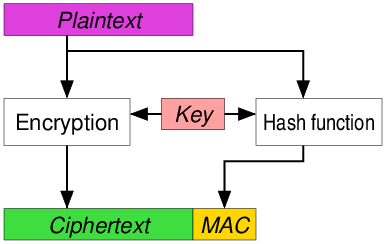
\includegraphics[scale=0.4]{screenshots/Authenticated_Encryption_EaM.png}
        \end{center}
    \end{parag}
	\begin{parag}{MAC then encrypt}
	    \begin{itemize}
	        \item $\times$ No integrity of ciphertext (in theory) it is possible to change ciphertext and have a valid MAC
	        \item \checkmark Integrity of the plaintext can be verified
	        \item \checkmark No information on the plaintext either, since it is encrypted
	    \end{itemize}
	    \begin{center}
	    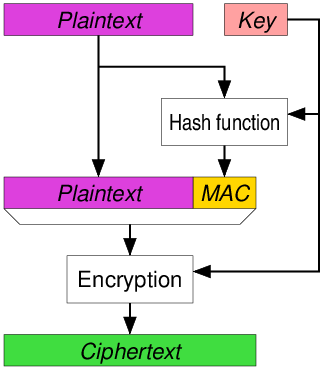
\includegraphics[scale=0.4]{screenshots/Authenticated_Encryption_MtE.png}
	    \end{center}
	\end{parag}
	\begin{parag}{Encrypt then MAC}
	    \begin{itemize}
	        \item \checkmark Integrity of ciphertext $\to$ ensures you only read valid massages! Cipher cannot be attacked!
	        \item \checkmark Integrity of the plaintext can be verified
	        \item \checkmark No information on the plaintext either, since it is encrypted
	    \end{itemize}
	    \begin{center}
	    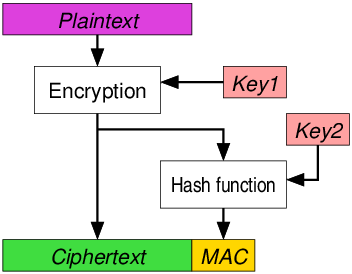
\includegraphics[scale=0.4]{screenshots/Authenticated_Encryption_EtM.png}
	    \end{center}
	\end{parag}














